\documentclass[../main.tex]{subfiles}

\graphicspath{{../images/}}

\begin{document}
\pagestyle{fancy}
\chead{Module 3}
\rhead{Junseo Shin}
\lhead{CSE 4059}


\renewcommand{\thefigure}{\arabic{figure}}
\section*{Image Blur}

\subsection*{Questions}

\begin{enumerate}
    \item How many floating-point operations are being performed in your color
    conversion kernel? EXPLAIN.

    The kernel performs $(2 * \texttt{BLUR\_SIZE} + 1)^2 + 3$ floating-point operations:
    One float assignment for \texttt{pixVal},
    $(2 * \texttt{BLUR\_SIZE} + 1)^2$ floating-point operations for the nested for loop,
    and two float assignments for the division and cast at the end of the function.

    \item How many global memory reads are being performed by your kernel?
    EXPLAIN.

    The kernel performs $(2 * \texttt{BLUR\_SIZE} + 1)^2$ global memory reads in the
    nested for loop every time we call for the input image data.

    \item How many global memory writes are being performed by your kernel?
    EXPLAIN.

    The kernel performs one global memory write for each thread at the end of the function as
    we write the blurred pixel value to the output image.

    \item Describe what possible optimizations could be implemented to your kernel
    to achieve a performance speedup.

    Once again, we can use block sizes that are a multiple of the warp size (32) and use
    shared memory to reduce the number of global memory reads and writes especially in the
    nested for loop where we are averaging the pixel values.
\end{enumerate}

% \newpage

\begin{figure}
    [ht]
    \centering
    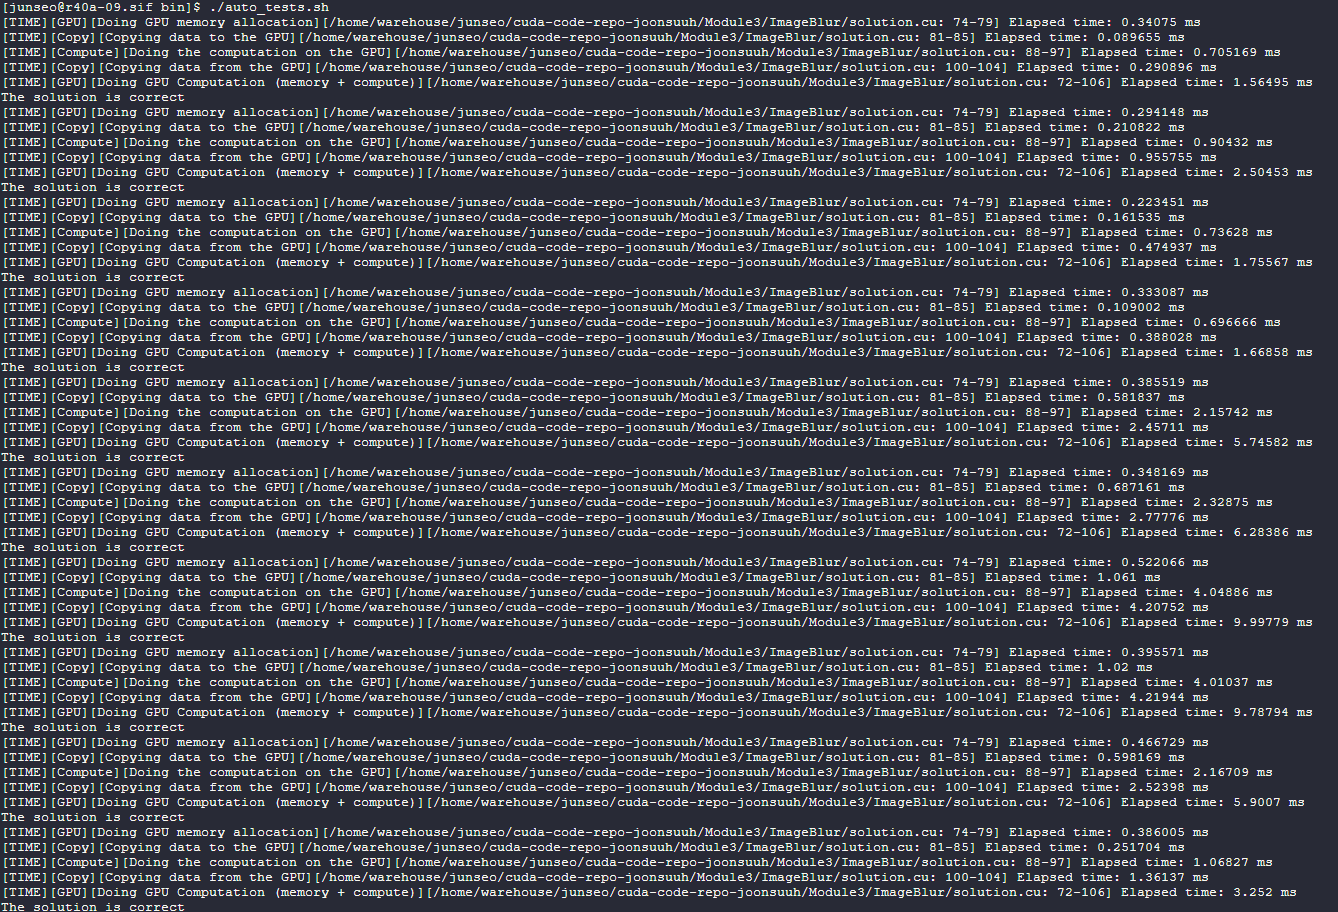
\includegraphics[width=1\textwidth]{imageblur.png}
    \caption{\texttt{ImageBlur\_Solution} output}
\end{figure}
\end{document}